%Auteurs : Nicolas Englebert
\documentclass[british,french,11pt, a4paper, openany]{book}

% Règles de bonne pratiques :
% https://fr.wikibooks.org/wiki/LaTeX/Gestion_des_gros_documents
\usepackage{../../Builder/preambule}
% %%%%%%%%%%%%%%%%
%%% Packages %%%
%%%%%%%%%%%%%%%%

%%% Compatibilité %%%
\begingroup\expandafter\expandafter\expandafter\endgroup
\expandafter\ifx\csname IncludeInRelease\endcsname\relax
\usepackage{fixltx2e}
\fi 					% Si version LaTeX < 2015, inclut un fix.

%%% Général %%%
\usepackage[utf8]{inputenc}
\usepackage{babel}
\usepackage{lmodern}
\usepackage[T1]{fontenc}
\addto\extrasfrench{\sisetup{locale = FR,detect-all}} % Switch siunitx en fonction de la langue babel :)
\addto\extrasbritish{\sisetup{locale = UK,detect-all}}
\usepackage{courier}
\usepackage{graphicx}
%\usepackage{cancel}

%%% Tableau %%%
%\usepackage{tabularx} %Permet d'auto dimensionner les tableaux



%%% Bibliographie %%%
%\usepackage[style=alphabetic,backend=biber]{biblatex}
\usepackage[autostyle]{csquotes}
%\DeclareNameAlias{sortname}{last-first}
%\DeclareFieldFormat{url}{\space\url{#1}}
%\DeclareNameAlias{labelname}{last-first}
%\addbibresource{sample.bib}


%%% Graphiques %%%
%\usepackage{tikz}
%\usepackage{pgfplots}
%\usepackage{circuitikz}

%%% Mise en page %%%
\usepackage{mathtools}
\usepackage{amssymb}
\usepackage{bbm}
\usepackage{amsthm}
%\usepackage[tt]{titlepic}% Centre le titre
%\usepackage{fancyhdr}   % Permet de modifier l'entête & footer
\usepackage{caption}     % Permet d'ajouter des légendes en images sans les mettre en float + dans la marge + ref vers le haut de l'envirronement
\usepackage{wrapfig}
\usepackage{fullpage}
%\usepackage{multicol}   % pour les liste sur plusieurs colonnes
%\usepackage{subfigure}  % alligne deux images cote a cote
\usepackage{float}      %permet de mettre du texte entre les figures grace a [H]. Génial! 
\usepackage{eso-pic}    % Fond d'écran page de garde
\usepackage{adjustbox}  % Empêche les box de sortir de la page


%%% Math %%%
%\usepackage{delarray} % Belles matrices
\usepackage{siunitx}


%%% Codes %%%
%\usepackage{listings}
%\usepackage[final]{pdfpages} %% Inclusion fichier pdf

%% Reference
\usepackage{hyperref}
%\renewcommand*{\figureautorefname}{fig.}
%\def\appendixautorefname{annexe}
%\def\tableautorefname{tab.}
%\renewcommand*{\chapterautorefname}{ch.}
%\newcommand{\subfigureautorefname}{\figureautorefname}



%%%%%%%%%%%%%%%%%
%%% Commandes %%%
%%%%%%%%%%%%%%%%%

%%% Physique %%%
\newcommand{\cst}{\text{cst}}
\newcommand{\D}{\partial}
\newcommand{\E}{\vec E}
\newcommand{\B}{\vec B}
\newcommand{\F}{\vec F}
\newcommand{\modu}[1]{|$#1$|}

%%% Math %%%
\newcommand{\oiint}{\int\!\!\!\!\!\!\! \:\!\subset\!\!\supset\!\!\!\!\!\!\!\int}
\newcommand{\rot}{\operatorname{\vec{rot}}}
\newcommand{\divv}{\operatorname{div}}
\newcommand{\phas}[1]{\underline{#1}}
\newcommand{\RE}{\text{Re}}
\newcommand{\ft}{\overset{\mathcal{F}}{\longleftrightarrow}}
\newcommand{\lt}{\overset{\mathcal{L}}{\longleftrightarrow}}
\newcommand{\DS}{\displaystyle}
\newcommand{\Tr}{\operatorname{Tr}}



%% Box
\shorthandon{:}
\newcommand{\theor}[1]{\adjustbox{minipage=\linewidth-2\fboxsep-2\fboxrule,fbox}{\textsc{\iflanguage{british}{Theorem}{Théorème}: }#1}}
\newcommand{\defi}[1]{\adjustbox{minipage=\linewidth-2\fboxsep-2\fboxrule,fbox}{\textsc{\iflanguage{british}{Definition}{Définition}: }#1}}
\newcommand{\lemme}[1]{\adjustbox{minipage=\linewidth-2\fboxsep-2\fboxrule,fbox}{\textsc{\iflanguage{british}{Lemma}{Lemme}: }#1}}
\newcommand{\prop}[1]{\adjustbox{minipage=\linewidth-2\fboxsep-2\fboxrule,fbox}{\textsc{\iflanguage{british}{Property}{Propriété}}\\ #1}}
\newcommand{\proposition}[1]{\adjustbox{minipage=\linewidth-2\fboxsep-2\fboxrule,fbox}{\textsc{Proposition}\\#1}}
\newcommand{\cadre}[1]{\adjustbox{minipage=\linewidth-2\fboxsep-2\fboxrule,fbox}{#1}}
\newcommand{\retenir}[1]{\adjustbox{minipage=\linewidth-2\fboxsep-2\fboxrule,fbox}{\textbf{\textit{\textsc{\iflanguage{british}{To remember}{À retenir}}: }}#1}}

\newcommand{\corollaire}[1]{\bigbreak\begin{tabular}{||c}
	\begin{minipage}{\textwidth}
		\textsc{\iflanguage{british}{Corollary}{Corollaire}: } \textit{#1}
	\end{minipage}
	\end{tabular}}
\newcommand{\exemple}[1]{\bigbreak\begin{tabular}{|c}
	\begin{minipage}{\textwidth}
		\textsc{\iflanguage{british}{Example}{Exemple}: } #1
	\end{minipage}%
	\end{tabular}}%
\shorthandoff{:}
    

%\pagestyle{headings} % Titre du ch et numéro page dans l'entete
%\renewcommand{\proofname}{Démonstration}
%\addto\captionsfrench{\def\tablename{Tableau}}


%%% Background %%%
\newcommand\BackgroundPic{%
	\put(0,0){%
		\parbox[b][\paperheight]{\paperwidth}{%
			\vfill
			\centering
			\includegraphics[width=\paperwidth,height=\paperheight,%
			keepaspectratio]{../../Builder/ulb.jpg}%
			\vfill
}}}

%%% Annexes Cedu %%%
%\usepackage{calrsfs}
%\DeclareMathAlphabet{\pazocal}{OMS}{zplm}{m}{n}
\usepackage{fourier-orns}

\setlength{\parindent}{0pt} 

%%% Attributs %%%
\newcommand*{\NomduCours}[2]{\def\cours{#1}\def\memo{#2}}
\newcommand*{\annee}[2]{\def\adebut{#1}\def\afin{#2}}

\newcounter{auteurcnt}
\newcommand\addauteur[2]{%
	\stepcounter{auteurcnt}%
	\csdef{auteur\theauteurcnt}{\mbox{#1~\textsc{#2}}}}
\newcommand\getauteur[1]{%
	\csuse{auteur#1}}

\newcounter{illustrateurcnt}
\newcommand\addillustrateur[2]{%
	\stepcounter{illustrateurcnt}%
	\csdef{illustrateur\theillustrateurcnt}{\mbox{#1~\textsc{#2}}}}
\newcommand\getillustrateur[1]{%
	\csuse{illustrateur#1}}

\newcounter{rappeltheocnt}
\newcommand\addrappeltheo[2]{%
	\stepcounter{rappeltheocnt}%
	\csdef{rappeltheo\therappeltheocnt}{\mbox{#1~\textsc{#2}}}}
\newcommand\getrappeltheo[1]{%
	\csuse{rappeltheo#1}}

\newcounter{professeurcnt}
\newcommand\addprofesseur[2]{%
	\stepcounter{professeurcnt}%
	\csdef{professeur\theprofesseurcnt}{\mbox{#1~\textsc{#2}}}}
\newcommand\getprofesseur[1]{%
	\csuse{professeur#1}}

\newcounter{iter}²

% Attributs
\NomduCours{Analyse I}{MATH-H-100}
\addauteur{Nicolas}{Englebert}
\addprofesseur{Anne}{Delandtsheer}
\annee{2013}{2014}

% Document
\begin{document}
\def\equationautorefname~#1\null{%
	(#1)\null
}

%%%%%%%%%%%%%%%%%
% Préliminaires %
%%%%%%%%%%%%%%%%%
\frontmatter
\AddToShipoutPicture*{\BackgroundPic}

\begin{titlepage}
	\begin{center}	
			
		\newcommand{\HRule}{\rule{\linewidth}{0.5mm}}   			            %Titre en gros
		\includegraphics[width=0.55\textwidth]{../../Builder/titlepage/logo.pdf}~\\[1cm]				%Logo
			
			\textsc{\LARGE Université Libre de Bruxelles}\\[1.5cm]
			\textsc{\Large \iflanguage{british}{Summary}{Synthèse}}\\[0.5cm]
			
			\HRule \\[0.4cm]
			{ \huge \bfseries \cours \ \\\memo \\[0.4cm] }
			
			
			\HRule \\[1.5cm]
			\begin{minipage}[t]{0.6\textwidth}
				\begin{flushleft}%\large
					\emph{\iflanguage{british}{Author}{Auteur}\ifnum\theauteurcnt>1 s\fi:}\\
					\whileboolexpr
					{ test {\ifnumcomp{\value{iter}}{<}{\theauteurcnt}} }%
					{\stepcounter{iter}\getauteur{\theiter}\\}
					\setcounter{iter}{0}%
					\ifnum\theillustrateurcnt>0%
					\ \\
					\emph{Illustrations:}\\
					\whileboolexpr
					{ test {\ifnumcomp{\value{iter}}{<}{\theillustrateurcnt}} }%
					{\stepcounter{iter}\getillustrateur{\theiter}\\}%
					\setcounter{iter}{0}%
					\fi%
					\ifnum\therappeltheocnt>0%
					\ \\
					\emph{\iflanguage{british}{Reminders}{Rappels théoriques}:}\\
					\whileboolexpr
					{ test {\ifnumcomp{\value{iter}}{<}{\therappeltheocnt}} }%
					{\stepcounter{iter}\getrappeltheo{\theiter}\\}%
					\setcounter{iter}{0}%
					\fi%
				\end{flushleft}
			\end{minipage}%
			\begin{minipage}[t]{0.25\textwidth}
				%\begin{flushright}
				%\large
				\emph{\iflanguage{british}{Professor}{Professeur}\ifnum\theprofesseurcnt>1 s\fi:}
				\whileboolexpr
				{ test {\ifnumcomp{\value{iter}}{<}{\theprofesseurcnt}} }%
				{\\ \stepcounter{iter}\getprofesseur{\theiter}}%
				\setcounter{iter}{0}%
				%\end{flushright}
			\end{minipage}
			
			\vfill
			
			% Bottom of the page
			{\large \iflanguage{british}{Year}{Année} \adebut~-~\afin}
			
		\end{center}
	\end{titlepage}

\ \\[2cm]
{\Huge \bfseries Appel à contribution}\\[5mm]
\subsection*{Synthèse Open Source}
\begin{wrapfigure}[5]{l}{4.5cm}
	\includegraphics[scale=0.5]{../../Builder/git.png}
\end{wrapfigure}
Ce document est grandement inspiré de l’excellent cours donné 
par \ifnum\theprofesseurcnt=1 \getprofesseur{1} \else\whileboolexpr
{ test {\ifnumcomp{\value{iter}}{<}{\theprofesseurcnt-2}} }%
{\stepcounter{iter}\getprofesseur{\theiter}, }%
\stepcounter{iter}\getprofesseur{\theiter} et \stepcounter{iter}\getprofesseur{\theiter} \fi%
 à l’EPB (École Polytechnique de Bruxelles), faculté de l’ULB (Université 
Libre de Bruxelles). Il est écrit par les auteurs susnommés avec l’aide de tous les autres étudiants 
et votre aide est la bienvenue ! En effet, il y a toujours moyen de l’améliorer surtout que si le 
cours change, la synthèse doit être changée en conséquence. On peut retrouver le code source à l’adresse 
suivante
\begin{center}
	\url{https://github.com/nenglebert/Syntheses}
\end{center}\bigskip
Pour contribuer à cette synthèse, il vous suffira de créer un compte sur \textit{Github.com}. De
légères modifications (petites coquilles, orthographe, ...) peuvent directement être faites sur le
site ! Vous avez vu une petite faute ? Si oui, la corriger de cette façon ne prendra que quelques 
secondes, une bonne raison de le faire ! \bigskip

Pour de plus longues modifications, il est intéressant de disposer des fichiers : il vous 
faudra pour cela installer \LaTeX, mais aussi \textit{git}. Si cela pose problème, nous sommes 
évidemment ouverts à des contributeurs envoyant leur changement par mail ou n’importe quel autre 
moyen.\bigskip

Le lien donné ci-dessus contient aussi un \texttt{README} contenant de plus amples informations, 
vous êtes invités à le lire si vous voulez faire avancer ce projet ! 

\subsection*{Licence Creative Commons}
\begin{wrapfigure}[3]{r}{2.8cm}
	\vspace{-5mm}
	\includegraphics[scale=0.17]{../../Builder/CC}
\end{wrapfigure}
Le contenu de ce document est sous la licence Creative Commons : \textit{Attribution-NonCommercial-ShareAlike 
4.0 International (CC BY-NC-SA 4.0)}. Celle-ci vous autorise à l'exploiter pleinement, compte-
tenu de trois choses :
\begin{enumerate}
	\item \textit{Attribution} ; si vous utilisez/modifiez ce document vous devez signaler le(s) nom(s)
	      de(s) auteur(s).
	\item \textit{Non Commercial} ; interdiction de tirer un profit commercial de l’œuvre sans 
	      autorisation de l'auteur 
	\item \textit{Share alike} ;  partage de l’œuvre, avec obligation de rediffuser selon la même 
	      licence ou une licence similaire
\end{enumerate}
Si vous voulez en savoir plus sur cette licence :
\begin{center}
	\url{http://creativecommons.org/licenses/by-nc-sa/4.0/}
\end{center}

\begin{flushright}
	\textbf{Merci ! }
\end{flushright}
\tableofcontents
%Si abstract, \input ici

%%%%%%%%%%%%%%%%%%%%%
% Contenu principal %
%%%%%%%%%%%%%%%%%%%%%
\mainmatter
\chapter{Topologie dans $\mathbb{R}$}
\section{Le champ ordonné R, +, .}
$\mathbb{R}$ est ordonné, c'est à dire qu'il est muni d'un ordre total.
\begin{equation}
	\left\lbrace
	\begin{array}{ccc}
		x \leq y \Rightarrow x + y \leq y+z      \\
		0 \leq x, 0 \leq y \Rightarrow 0 \leq xy \\
	\end{array}\right.
\end{equation}
\textit{Notons que le champ des complexes ne peut être ordonné}
\\
\subsection*{Axiome de Dedekind}
Le champ $\mathbb{R},+,.$ le satisfait : Il existe un \textit{point de démarcation} entre A et B tel que :
$$ \exists c \in \mathbb{R} : \forall a \in A, \forall b \in B \Rightarrow a \leq c \leq b $$
Ceci n'est pas d'application dans $\mathbb{N}$

\section{Complétion de $\mathbb{R}$ par $\pm \infty$}
Une demi droite fermée inférieurement sera dite \textit{minorée} tandis qu'elle sera dite \textit{majorée} si elle est bornée supérieurement.

\section{Ensemble borné}
A est dit borné ssi il est majoré \textbf{et} minoré : $\exists m, M \in \mathbb{R} : \forall a \in A, m \leq a \leq M$\\
On dit que $x$ majore A $\Leftrightarrow x \geq a \forall a \in A$
On dit que $x$ minore A $\Leftrightarrow x \leq a \forall a \in A$

\section{Infimum et suprémum}
On appelle $SupA$ la borne supérieure de A.\\
Toute partie non vide  majorée admet ainsi un \textit{Sup/Inf} dans $\mathbb{R}$.\\
\textbf{CNS:} Si $s$ majore A, alors $\forall \epsilon > 0, s- \epsilon $ ne majore pas A.\\
Notons que le suprémum existe toujours dans $\mathbb{R}$ achevé.

\section{Valeur absolue et inégalité triangulaire}
L'inégalité triangulaire s'exprime de la façon suivante :
$$ \forall x, y \in \mathbb{R} : |x| - |y| \leq |x + y| \leq |x| + |y| $$
Elle peut bien évidemment se généraliser en \textit{n} dimensions dans sa notation vectorielle.

\chapter{Limites}
\section{Limite infinie d'une fonction}
La définition de la limite d'une suite est la suivante :
$$ \forall \epsilon > 0, \exists r > a : x > r \Rightarrow |f(x) - l| < \epsilon $$
La limite d'une fonction existe si celle-ci $\in \mathbb{R}$

\section{Limite d'une suite}
Dans ce cas, la définiton devient :
$$ \forall \epsilon > 0, \exists N \in \mathbb{N}_{0} : n \geq N \Rightarrow |U_{n} - l| < \epsilon$$
Le but est de \textit{trouver} un $N$ (un seuil) à partir duquel toutes les valeurs de la suites sont identiques.\\


\section*{Calcul des limites de suites}
Le passage à la limite conserve les inégalités \textbf{non-strictes}.\\
Les suites de Fibonacci sont à lire à titre plutôt informatif.

\section*{Croissance et décroissance de suite}
Une suite sera dite \textit{bornée/majorée/minorée} si l'ensemble ${U_{n}}$ est borné/majoré/minoré.\\
\textbf{Implication:} Suite bornée $\Rightarrow$ convergence (réciproque fausse! Par exemple $(-1)^{n}$ est bornée mais ne converge pas.)\\

\begin{proof}
	
	$$Soit\ \epsilon = 1. On\ sait\ que\ \exists N : \forall n \geq N, U_{n} \in ]u-1, u+1[ $$
	$$Donc\ B:= {U_{n}, n \geq N}\ est\ borné$$
	$$Or\ F:= {U_{n}, n \leq U_{n-1}}\ est\ fini\ donc\ borné$$
	$$Donc\ B \cup F\ est\ bornée.$$
\end{proof}


$$(U_{n})\ est\ bornée\ \Leftrightarrow \exists M > 0 : |U_{n}| \leq\ M\  \forall n \in \mathbb{N}_{0} $$
Une suite est dite \textit{monotone} si elle est croissante \textbf{ou} décroissante.\\
Notons également que toute suite croissance majorée converge vers son suprémum dans $\mathbb{R}$

\begin{proof}
	$$Posons\ \sigma := sup(U_{n})$$
	$$\forall \epsilon > 0, \exists N : \forall \epsilon > 0, \sigma - \epsilon\ n'est\ pas\ marjorant\ : \exists U_{n} > \sigma - \epsilon$$
	$$Or\ U_{n}\ est\ croissante\ : \forall n \geq N : U_{n} > \sigma - \epsilon \Rightarrow \sigma - \epsilon < U_{n} < \sigma + \epsilon$$
	$$D'où\\ \lim\limits_{\substack{n \to \infty}} U_{n} = \sigma$$
\end{proof}

Une suite $(U_{n})_{n \in \mathbb{N}_{0}}$ est dite croissante ssi :
$$ U_{n} \leq U_{n+1}$$


\section{Comportement asymptotique}
\subsection{o, O, \string~ et comportement équivalent}
Deux suites ont le même \textit{comportement asymptotique} :
$$ U_{n} \text{\string~} V_{n} \Leftrightarrow \lim\limits_{\substack{x \to \infty}} \frac{U_{n}}{V_{n}} = 1 = \lim\limits_{\substack{x \to \infty}} \frac{V_{n}}{U_{n}} $$
Attention cependant, $|U_{n} - V_{n}| \nLeftarrow \nRightarrow \frac{U_{n}}{V_{n}} = 1$ (Prendre comme contre-exemple $x+2$ et $x$).
\\
\subsection*{Petit O}
$U_{n}$ est un petit o de $V_{n}$, c-à-d :\\ 
$$U_{n} = o(V_{n}) \Leftrightarrow \lim\limits_{\substack{x \to a}} \frac{U_{n}}{V_{n}} = 0\ pour\ x \rightarrow a$$
\subsection*{Grand O}
$U_{n}$ est un grand O de $V_{n}$, c-à-d :
$$U_{n} = O(V_{n}) \Leftrightarrow \exists c \in \mathbb{R}^{+}, \exists N : \forall n \geq N : |U_{n}| \leq C|V_{n}|\ pour\ x \rightarrow a$$ \\
Autrement dit, le rapport des limites est borné.\\
\textbf{Attention : } Petit O et grand O ne sont pas symétrisable, ni des relation d'indépendance.\\
\\
\textit{NB : Ces notions sont aussi d'application pour les fonctions, elles ne concernent pas uniquement les suites.}

\subsection{Complexité d'algorithmes}
Deux algorithmes ont une complexité équivalente s'ils comportent le même nombre d'étapes.

\subsection{Courbes asymptotes au graphe de $f$}
La \textit{droite} $y = ax + b$ est asymptote au graphe de $f$ pour $x \rightarrow \infty$ 
$$ \Leftrightarrow \lim\limits_{\substack{x \to \infty}} (f(x) - (ax+b)) = 0$$
La \textit{courbe} $y=g(x)$ est asymptote au graphe de $f$ pour $x \rightarrow \infty$ 
$$ \Leftrightarrow \lim\limits_{\substack{x \to \infty}} (f(x) - g(x)) = 0$$

\subsection{Suite partielle, queue de suite}
Soit $(n_{k})$ une suite strictement croissante de nombre naturels. Alors la suite $(U_{nk})$ est appelée \textit{suite partielle} (ou \textit{sous-suite}) de la suite $(U_{n})$

\subsection{Limites sup et inf}
Il s'agit de la plus grande et de la plus petite suite partielle \textbf{convergente} d'une suite. Elles se définissent telle que :
$$ \lim\limits_{\substack{x \to \infty}} sup\ U_{n} = \lim\limits_{\substack{x \to \infty}} (sup\ {U_{n} : n \geq s})$$
$$ \lim\limits_{\substack{x \to \infty}} inf\ U_{n} = \lim\limits_{\substack{x \to \infty}} (inf\ {U_{n} : n \geq s})$$
La convergence d'une suite est caractérisée par la coïncidence de ses \textit{liminf} et \textit{limsup}. Si celles-ci ne sont pas identique, la suite diverge.\\
On peut donc en tirer :\\
\begin{center}
	\textit{Si une suite converge, l'ensemble de ses sous-suites converge vers la même valeur.}
\end{center}

\subsection{Limites d'une fonction en un point réel}
La limite de $f$ pour $x \rightarrow a$ existe ssi il existe $l \in \mathbb{R}$ tel que : 
$$\forall \epsilon, \exists \delta > o : |x-a| < \delta\ (x \in A) \Rightarrow |f(x) - l| < \epsilon$$

\section{Continuité, discontinuité}
La fonction $f$ est \textit{continue} en a ssi $\lim\limits_{\substack{x \to a}} f(x) = f(a)$. \\
On dira ainsi que $f$ est discontinue si elle n'est pas continue en a. Plus formellement : 
$$\forall \epsilon, \exists \delta > o : |x-a| < \delta (x \in A) \Rightarrow |f(x) - f(a)| < \epsilon$$

\subsection{Espèces de discontinuité}
La limite à gauche et à droite existent mais sont différentes, on parle de \textit{discontinuité de première espèce}.\\
On parlera de \textit{discontinuité de deuxième espèce} si la limite à gauche ou à droite n'existe pas.

\subsection{Fonction croissante et décroissante}
f est croissante $\Leftrightarrow x < y \Rightarrow f(x) \leq f(y)$\\
f est strictement croissante $\Leftrightarrow x < y \Rightarrow f(x) < f(y)$\\
f est décroissante $\Leftrightarrow x < y \Rightarrow f(x) \geq f(y)$\\
f est croissante $\Leftrightarrow x < y \Rightarrow f(x) > f(y)$\\
Si $f$ est strictement monotone, alors $f$ est \textit{injective} ($\nLeftarrow$)

\subsection{Suprémum d'une fonction}
Le \textit{suprémum} de f : $sup\ f := sup{f(x) | x \in A}$

\subsection{Discontinuité des fonctions monotones}
Toute discontinuité d'une fonction \textit{monotone} sur un \textbf{intervalle} au sens large est de première espèce.

\chapter{Fonction continue}
\section{Ensemble de niveau, image fonction réciproque}
On définit la réciproque telle que $f^{-1} (c) := {x \in A ; f(x) = c}$.\\
Pour que $f$ admette une fonction réciproque il faut que celle-ci soit injective (Par rapport à \textit{Connaissances fondamentales}, il faut bien qu'elle soit bijective mais.. sur son image!)

\section{Fonctions élémentaires}
Il s'agit de cinq fonctions qui sont toujours continue sur leur domaine (Fonction constante, identité, sinus, exponentielle, $x^{n}$).\\
\textbf{Attention :} Bien que je ne les mentionne pas ici, il faut connaître un minimum les fonctions hyperboliques (\textit{section 3.2.7 du syllabus})

\section{Image d'un intervalle par une fonction continue}

\subsection{Théorème de la valeur intermédiaire (TVI)}
\textit{L'image d'un intervalle par une fonction continue est un intervalle}.\\
On dira que $f$ est \textit{connexe} $\Leftrightarrow \forall a, b \in E : a < c < b où c \in E$\\\\

On peut ré-exrprimer le TVI de la façon suivante : \textit{Si $[a,] \in domf \rightarrow $ toute valeur intermédiaire entre $f(a)$ et $f(b)$ est atteinte au moins une fois par f entre a et b}.
\subsection*{Application du TVI}
$$Si\ sign((f(a))\ \neq\ sign(f(b))\ \Rightarrow \exists x \in ]a, b[ : f(x) = 0$$

\section*{Racine d'un polynôme de degré impair}
Tout polynôme à coéfficients réels et de degré impair possède au moins une racine réelle.

\begin{proof}
	$$Soit\ P(x) = a_{m}x^{m} + ... + a_{1}x + a_{0} = x^{m}(a_{m} + \sum_{i=0}^{m-1} \frac{a_{i}}{x^{m-1}})\ où\ m\ est\ impair\ et\ a_{m} > 0$$
	$$Comme \lim\limits_{\substack{x \to \infty}} \frac{1}{x^{n}} = 0\ (Si\ n > 0) $$
	$$ \lim\limits_{\substack{x \to \infty}} P(x) = \pm \infty$$
	$$ \Rightarrow x_{1}, x_{2} \in \mathbb{R} | P(x_{1}) > 0, P(x_{2}) < 0$$
	$$Comme\ P(x)\ est\ continue,\ il\ suffit\ de\ lui\ appliquer\ le\ TVI.$$
\end{proof}

\subsection{Théorème du point fixe}
Si $f: [a,b] \Longrightarrow [a,b]$ est continue, alors $f$ admet au moins un point fixe ($f(p) = p$).\\
\begin{proof}
	Il suffit d'appliquer le Th. de la valeur intermédiaire à la fonction auxiliaire $g$ définie par $g := x-f(x)$
	$$g(x) = a - f(a) < 0 < b - f(b) = g(b)$$
	Donc par le TVI : $$\exists p \in [a,b] = g(p) = 0 \Rightarrow f(p) = p$$
\end{proof}

\section{Image d'un compact par $f$ continue}
Les qualités \textbf{non préservées} par une fonction continue sont : être ouvert, fermé et borné.\\
Les qualités \textbf{préservées} par une fonction continue sont : être connexe, être compact (= fermé et borné).

\subsection{Existence du maximum de f}
Si est est continue sur un intervalle fermé (compact) alors la fonction continue admet un \textit{minimum} et un \textit{maximum}

\subsection{Maximants}
Un point $x \in A$ : f(x) = max(f(a)) = \textit{maximant}\\
Un point $x \in A$ : f(x) = min(f(a)) = \textit{minimant}\\\
\textbf{Attention :} Ne pas confondre maximum et maximant. Une fonction peut avoir une infinité de maximants mais jamais plus d'un maximum.



\chapter{Dérivée et différentielle}
\section{Dérivée en un point}
On appelle le \textit{quotient différentiel} : $\frac{\Delta f}{\Delta X} = \frac{f(x) - f(a)}{x - a}$. \\
Si la limite existe en ce point a, la fonction est dite \textit{dérivable au point}.
\textbf{Attention :} f est dérivable en a $\Leftrightarrow$ les dérivées à gauche et à droite existent et sont identiques !

\subsection*{Dérivable implique continue}
Si f est dérivable en a $\Rightarrow$ f est continue en a ($\nLeftarrow$). On peut prendre comme contre-exemple la fonction valeur absolue. 

\begin{proof}
	Par hypothèse $\lim\limits_{\substack{n \to a}} \frac{f(x)-f(a)}{x-a}$ existe dans les réels.\\
	Or, le démominateur tend vers 0, le numérateur doit également tendre vers 0, c-à-d que f doit être continue en a.\\
	Si f(x) ne tend pas vers f(a) lorsque $x \rightarrow a $, alors la limite ne peut exister.
\end{proof}

\section{Différentielle en un point}
La différentielle $df$ est une application/fonction : $df := f'(x_{0}).\Delta x$ (Soit la pente * accroissement)\\
\textbf{Attention :} il ne faut pas la confondre avec la dérivée qui est un nombre.\\
Cette différentielle peut correspondre à un accroissement de f en un point. \\
Deux proproétés importantes :
\begin{itemize}
	\item C'est une application linéaire $\mathbb{R} \rightarrow \mathbb{R}$
	\item $f(x) - f(a) - df_{a}(x-a) = o(x-a)\ pour\ x \rightarrow a$
\end{itemize}

\section{Règle de calcul de dérivées, différentielles}
\subsection{Dérivée d'une composée}
La démonstration est à connaître.\\
\textit{NB : } Une fonction dérivée n'est pas forcément continue. Pour faire 'le tri', on définit les classes $C^{k}$ qui signifie : \textit{k fois dérivable ET continue}

\section{Dérivée en un extrémant local}
(\textit{Soit $ f : A \subseteq \mathbb{R} \rightarrow \mathbb{R}$}\\
On nomme \textit{maximum local} : Il existe un voisinage V de $\tilde{x}$ tel que $\forall x \in V \\bigcap A : f(x) \leq (\geq) f(\tilde{x})$\\
Alors $\tilde{x}$ est dit \textit{extrémant}.

\subsection{CN d'ordre 1 pour un extrémant local libre}
Si $\tilde{x} \in$ Int A est un extrémant local de $f$ et $f$ est dérivable en $\tilde{x}$, alors $f'(\tilde{x}) = 0$\\
\begin{proof}
	$$f'(a) = \lim\limits_{\substack{x \to a^{+}}} = \frac{f(x) - f(a)}{x-a} \leq 0$$
	$$f'(a) = \lim\limits_{\substack{x \to a^{-}}} = \frac{f(x) - f(a)}{x-a} \geq 0$$
\end{proof}

\subsection{Point critique, point suspect}
Soit $x \in$ Int A est un \textit{point critique} si $f'(x) = 0$\\
Un point est dit \textit{suspect} (C'est à dire "candidat" pour être un extrémum s'il fait partie d'une des trois "listes" suivantes :
\begin{itemize}
	\item $f'(c) = 0$
	\item $f'(c) \nexists$
	\item $c \in A\backslash Int A$ (Si $c$ est un bord)
\end{itemize}

\section{Formule des accroissements finis}
Si $f: [a,b] \rightarrow \mathbb{R}$ est \textit{continue} sur [a,b] \textbf{et} \textit{dérivable} sur ]a,b[ alors : \\
$$\exists c \in ]a,b[ : f'(c) = \frac{f(b)-f(a)}{b-a}$$
\begin{proof}
	Il suffit d'appliquer le théorème de Rolle à la fonction auxiliaire $g$ définie comme : 
	$$g : [a,b] \rightarrow \mathbb{R} : x \rightarrow f(x) - f(a) - \frac{f(b) - f(a)}{b-a}(x-a)$$
\end{proof}

\subsection{Théorème de Rolle}
Les pré-requis sont les mêmes que pour le Th. des accroissements fini. Il faut néanmoins ajouter : $f(a) = f(b)$. On a alors :
$$\exists c \in ]a,b[ : f'(c) = 0 $$
\begin{proof}
	$f \in C^{0}$ sur [a, b], par le théorème des valeurs extrèmes. Il existe un $x_{M}$ et $x_{m}$  dans [a,b] tels que : 
	$$f(x_{M}) = max(f(x))\ et\ f(x_{m}) = min(f(x))$$
	Si les extrémants $x_{M}$ et $x_{m}$ ne sont pas intérieur à [a,b] :
	$$f(a) = f(b) = min(f(x)) = max(f(x)) \Rightarrow f(x)\ est\ constante\  \Rightarrow f'(x) = 0$$
	Si les extrémants ne sont pas intérieurs à [a,b], alors $f'(x) = 0$
\end{proof}



\section{Les primitives}
Si : 
\begin{itemize}
	\item $f' = 0$ sur un intervalle I, alors f est constante sur I
	\item Si $f$ et $g$ ont la même dérivée, alors $f$ et $g$ diffèrent à une constante près
\end{itemize}
\begin{proof}
	Par hypothèse, $f$ est dérivable sur I. Soient $a, b \in I$. Par la formule des accroissements finis, il existe $c \in ]a, b[$ tel que :
	$$f(b) - f(a) = f'(c)(b-a) \Rightarrow f(b) = f(a)$$
\end{proof}
On définira la primitive : $f:A \subseteq \mathbb{R} \rightarrow \mathbb{R}$ , une primitive de $f$ est une fonction $F$ telle que $\forall x \in A : F'(x) = f(x)$

\section{Règle de l'Hospital}
Il faut que $f$ et $g$ soit dérivables sur un \textit{voisinage épointé autour de a} sans quoi on pourrait se trouver dans le cas d'une hospitalisation intempestive.

\section{Développement de Taylor}
Un approche de degré un sera dite \textit{affine}. Pour les degrés supérieurs, on parle de \textit{développement de Taylor} (Ou MacLaurin si autour de 0).
\begin{center}
	Le développement limite (de Taylor- de f, d'ordre k, près de a, est le polymome $P_{k}$ de degré $\leq k | e(x) = f(x) - P(x-a) = o((x-a)^{k})\ pour\ x \rightarrow a$
\end{center}
Cela signifie que l'erreur de l'approximation de f est d'ordre $k$ et que celle-ci tend plus vite vers 0 que l'approximation. On dira ainsi qu'une meilleure approximation est une approximation dont l'erreur tend plus vite vers 0.\\
\textbf{Attention :} Ne pas oublier de préciser pour $x \rightarrow a$ à la fin de l'approximation.

\subsection{Formule du reste de Lagrange}
Si $f \in C^{k+1}$, on peut définir l'erreur commise :
$$\exists c : x < c < a\ |\ R_{f, a, k}(x) = \frac{f^{k+1}(c) . (x-a)^{k+1}}{(k+1)!}$$
\textit{NB : } Pour $k=0$, on retrouve le Th. des accroissements finis!\\\\

Notons que le reste peut également être majoré : $|R_{f, a, k}(x)| = \frac{C|(x-a)^{k+1}|}{(k+1)!}$\\\\
On peut en tirer le corrolaire suivant : \\
Si $f^{k+1}$  est bornée au voisinage de a, alors : 
$$R_{f, a, k}(x) = o(|x-a|^{k})\ pour\ x \rightarrow a $$

\section{Croissance de f est signe de sa dérivée}
\subsection{Croissance et dérivée positive}
Si $f$ est dérivable sur ]a,b[ $\rightarrow$ $f$ est croissante sur ]a,b[ $\rightarrow f' \geq 0$ (sur ]a,b[, $\forall x \in ]a,b[$)\\
La démonstration est à connaître.

\subsection{Test de la première dérivée non nulle}
Soit $f:]a,b[ \rightarrow \mathbb{R}$ une fonction de classe $C^{k}$ et soit $\tilde{x} \in ]a,b[$\\
Supposons que $f'(\tilde{x}) = f''(\tilde{x}) = ... = f^{k-1}(\tilde{x}) = 0 $ et $f^{k}(\tilde{x}) \neq 0$\\ Alors : 
\begin{itemize}
	\item Si $k$ est pair, il s'agit d'un point d'extrémum local strict si $f^{k}(\tilde{x}) >(<) 0 $
	\item Si $k$ est impair, alors $\tilde{x}$ n'est pas un point d'extrémum local strict.
\end{itemize}
On peut également dire que le point $(\tilde{x}, f(\tilde{x}))$ est un point d'inflexion à tangente horizontale du graphe de f.


\chapter{Chapitre supprimé}
\chapter{Équations différentielles}
\section{Exemple}
\subsection{Primitives}
Soit $y' = f(x)$, une \textit{équation différentielle} d'ordre 1. Les solutions sont : $y : x \rightarrow y(x)$\\
Géométriquement, on impose une pente en tout point d'abcisse x. On désigne cela de \textit{champ de pente}.\\
Les courbes à même pentes sont dites \textit{isoclines} et la \textit{courbe intégrale} représente le graphe de toutes les solutions.

\section{Définition et approche qualitatives}
\section{EDO}
La solution de l'ED s'exprime : $fct : x \rightarrow y(x) : y' = f(x, y(x))\ \ (\forall x \in dom\ y)$. Il y en a une infinité.\\
On parle de \textit{problème de Cauchy} lorsqu'il faut trouver une solution satisfaisant des conditions initiales.

\subsection{Équations à variables séparées}
Nous parlons d'une équation du type : $y' = f(x).g(x)$. dont la solution est : $$\forall x \in I, \frac{d \phi}{dx}(x) = f(x).g(\phi (x))$$
Si $g$ est constante, la solution sera représentée par des droites isoclines verticales. Ces droites seront horizontales si $f$ est constante.\\
La combinaison de ces deux types de solutions donna la courbe intégrale. 

\subsection{ED à VS : Cas général}
Il suffit d'utiliser la "recette"; \textit{Cf. TP 7}.

\subsection{Problème de Cauchy}
Problème satisfaisant des conditions initiales. Deux propositions sont remarquables dans le cas ; $y' = f(x).g(x), y(x_0) = y_0$ :
\begin{enumerate}
	\item Si $g(y_0) \neq 0$, alors il existe un voisinage de $(x_0,y_0)$ dans lequel ce problème de Cauchy admet une et une seule solution.
	\item Si $g$ ne s'annule pas sur son domaine, alors ce problème de Cauchy admet une et une seule solution $\phi : I \rightarrow \mathbb{R}$, \textit{"maximale"} et \textit{"s'étendant d'un bord à l'autre} du pavé $dom\ f\ \times\ dom\ g$.
\end{enumerate}

\section{Équations différentielles linéaires (EDL)}
\subsection{Opérateurs différentiels linéaires}
\subsection{EDL d'ordre $n$}
Une équation \textit{différentielle linéaire} du $n^e$ ordre est une équation du type : 
$$a_n(x)y^n + a_{n-1}(x)y^{n-1} + ... + a_1(x)y' + a_0(x)y = b(x)\ \ \ \ \ \ \ \ \ \ \ \ \ (E_b)$$
L'équation \textit{homogène associée} est : 
$$a_n(x)y^n + a_{n-1}(x)y^{n-1} + ... + a_1(x)y' + a_0(x)y = 0\ \ \ \ \ \ \ \ \ \ \ \ \ \ \ \ \ (E_0)$$
Notons que \textit{l'ensemble des solutions de $E_0$ est un sous-vectoriel de $C^n$}.

\subsection{SGEnH = SGEH + SPEnH}
La solution générale de l'équation non homogène est égale à la solution générale de l'équation homogène associée plus une solution particulière de l'équation non homogène en question.

\subsection{Solution générale d'une EDL homogène d'ordre 1}
Soit l'EDL du $1^{er}$ ordre ($E_b$) et son équation homogène associée ($E_0$):
$$y' + a(x)y = b(x)\ \ \ \ \ (E_b)\ \ \ \ |\ \ \ \ y' + a(x)y = 0\ \ \ \ \ (E_0)$$
\textbf{Proposition :}\\
$y$ est solution de $E_0$ sur $I \subseteq \mathbb{R} \Leftrightarrow \exists c \in \mathbb{R} : \forall x \in I : y(x) = ce^{-A(x)}$.
\begin{proof}
	\ \\
	Posons $y(x) = c(x)e^{-A(x)}$ de sorte que $y' = c'e^{-A} - c\underbrace{A}_{=\ a}e^{-A}$\\
	On a alors (en remplaçant dans $E_0$)  :\\
	$$\Leftrightarrow c'e^{-A} - cae^{-A} + ace^{-A} = 0$$
	$$\Leftrightarrow c(x)\underbrace{e^{-A(x)}}_{\neq 0} = 0 \Leftrightarrow c' = 0 \Leftrightarrow c = c^{te}$$
\end{proof}
\textbf{Corollaire :}\\
L'ensemble des solutions de $E_0$ est un sous-espaces vectoriel de dimension 1 de l'espace vectoriel réel des fonctions dérivables.

\subsection{Variation de la constante}
Il s'agit d'une méthode consistant à rechercher les solutions d'une EDL d'ordre 1 sous la forme $c(x)e^{-A(x)}$ en remplaçant la constante par une fonction inconnue $c(x)$. (La méthode se généralise à l'ordre $n$. (\textit{Cf. TP 9}).

\subsection{Existence et unicité globale}
Tout problème de Cauchy pour l'EDL du $1^{er}$ ordre $y'+a(x)y = b(x)$, où $a, b \in C^0(I, \mathbb{R})$, admet une et une seule solution sur $I$.

\section{Réduction du $2^e$ ordre au $1^{er}$}
Méthode pratique, \textit{cf. Analyse I, 6.9}.

\section{EDLH du $2^e$ ordre à coefficients constants}
EDLH est l'abréviation d'Equation Différentielle Linéaire Homogène de la forme :
$$y'' + a_1y' + a_0y = 0\ \ \ \ \ \ \ \ (E_h)$$
\subsection{L'espace vectoriel des solutions}
La dimension de l'espace vectoriel vaut l'ordre de $E_h$.

\subsection{Rappel pour l'ordre 1}
Monte, feignant !

\subsection{Équation caractéristique}
Cherchons les solution de $E_h$ d'ordre 2 du type $y(x) = e^{\lambda x}$\ \ \ ($\lambda$ = constante).\\
$$\Leftrightarrow e^{\lambda x}(\lambda^2 + a_1\lambda + a_0) = 0$$
$$\Leftrightarrow \underbrace{\lambda^2 + a_1\lambda + a_0}_{polynôme\ caractéristique} = 0\ \ \ \Rightarrow EC$$
$$\Leftrightarrow \lambda = \frac{-a_1 \pm \sqrt{\Delta}}{2}$$
La nature des solution dépend du signe de $\Delta$.

\subsection{Racines réelles distinctes}
Si $\Delta > 0$, nous avons deux racines réelles : $\lambda_1$ et $\lambda_2$.\\La solution générale de $E_h$ s'écrit :
$$S.G.E.H.\ \ y(x) = c_1e^{\lambda_1 x} + c_2e^{\lambda_2 x}\ \ où\ c_1, c_2 \in \mathbb{R}$$

\subsection{Racines complexes conjuguées distinctes}
Si $\Delta < 0$, nous avons deux racines complexes : $\lambda_1 = \alpha +i\beta$ et $\lambda_2 = \alpha -i\beta$.\\
La solution générale de $E_h$ s'écrit :
$$S.G.E.H.\ \ y(x) = c_1e^{\alpha x} cos(\beta x) +c_2e^{\alpha x} sin(\beta x)\ \ où\ c_1, c_2 \in \mathbb{R}$$
\textit{NB :} Pour comprendre comment on se débarrasse de la partie imaginaire, consultez la section 6.10.5.

\subsection{Racines confondues}
Si $\Delta = 0$, nous avons une racine double (de multiplicité 2) : $\lambda = -\frac{a_1}{2}$. Comme l'ensemble des solutions doit être un EV de dimension 2 (ordre 2), on va multiplier cette racine par $x$ afin de trouver une deuxième solution linéairement indépendante.\\
La solution générale de $E_h$ s'écrit :
$$S.G.E.H.\ \ y(x) = e^{\lambda x}(c_1 + c_2x)\ \ où\ c_1, c_2 \in \mathbb{R}$$ 

\textit{NB :} La \textit{multiplicité} est le nombre de fois qu'une racine apparait. 

\subsection{Parties réelles et imaginaires de solutions complexes}
Dans le cas ou $\lambda_1$ et $\lambda_2$ sont deux complexes conjugués distincts, nous avons que :
$$y_1 = Re\ z_1\ \ \ et\ \  \ y_2 = Im\ z_1$$
Ceci illustre un fait plus général énoncé par \textbf{Lemme} :\\
Si $E_0$ est une EDO \textbf{linéaire homogène à coefficients réels} et si $z : I \subseteq \mathbb{R} - \mathbb{C}$ est une solution de $E_0$, alors les parties réelle et imaginaire Re $z$ et Im $z$ sont également solution de $E_0$.

\section{EDL non homogène du second ordre}
Il s'agit d'une équation du type : 
$$y'' + a_1y' + a_0y = b(x)\ \ \ \  (E_b)$$

\subsection{Méthode de la variation des constantes}
Comme énoncé ci-dessus, c'est principalement pratique : \textit{cf. TP 9}

\subsection{Quelques avantages de la linéarité}
Le principal avantage est que l'ont peut sommer les solutions générales de $y_1$ et $y_2$ pour avoir la solution générale de $y_1 + y_2$.

\subsection{Méthode des coefficients indéterminés}
Il s'agit de la méthode enseignée au \textit{TP 8}. Comme un aide mémoire de l'utilisation de la méthode est fourni à l'examen, je ne vais pas le recopier ici ! \\
L'aide mémoire est disponible sur l'UV et sur la deuxième de couverture du syllabus d'\textit{Analyse I, Chapitres 6 \& 7}.

\chapter{Fonctions à valeurs complexes et vectorielles}
Le chapitre a été passé. (Pour l'instant ?)

\chapter{Fonctions de plusieurs variables}
\section{Exemples et représentations géométriques}
Il s'agit des 38 premières pages du syllabus, elles sont données à titre informatif.

\section{Limite et continuité locale}
\subsection{Limite d'une fonction en un point}
Définition :\\
Soit $\vec{f} : A \subseteq \mathbb{R}^n \rightarrow \mathbb{R}^m$ et soit $\vec{a} \in adh A$. $\vec{f}$ \textbf{possède une limite} lorsque $\vec{x}$ (variant dans $A$) tend vers $\vec{a}\ (\in \mathbb{R}^n) \Leftrightarrow$
$$\exists \vec{l} \in \mathbb{R}^m : \lim\limits_{\substack{\vec{x} \to \vec{a}}} \vec{f}(\vec{x}) = \vec{l}$$
$$\Leftrightarrow$$
$$\exists \vec{l} \in \mathbb{R}^m : \forall \epsilon > 0, \exists \delta > 0 : ||\vec{x} - \vec{a}|| < \delta \}\Rightarrow ||\vec{f(x)} - \vec{l}|| < \epsilon$$
Il faut bien évidement que $\vec{a} \in adh\ domf$ pour que l'on puisse tendre vers celui-ci. Notons aussi que $\vec{l}$ doit exister dans l'\textit{espace d'arrivée}.

\subsection{Continuité d'une fonction en un point (de son domaine)}
Soit $\vec{f} : A \subseteq \mathbb{R}^n \rightarrow \mathbb{R}^m$ et soit $\vec{a} \in A.\ \vec{f}$ est \textbf{continue} \emph{en} $\vec{a} \Leftrightarrow$
$$\lim\limits_{\substack{\vec{x} \to \vec{a}}} \vec{f}(\vec{x}) = \vec{f}(\vec{a})$$
$\vec{f}$ est continue (\emph{sur} A) $\Leftrightarrow \forall\vec{a} \in A, \vec{f}$ est continue en $\vec{a}$. Cela revient à dire que $f$ est continue sur chacune de ses composantes.

\subsection{Limites composantes par composantes}
$$\lim\limits_{\substack{\vec{x} \to \vec{a}}} \vec{f}(\vec{x}) = \vec{l} \Leftrightarrow \forall i = 1, ..., m = \lim\limits_{\substack{\vec{x} \to \vec{a}}} \vec{f_i}(\vec{x}) = l_i$$
\begin{center}
	et $\vec{f}$ est continue en $\vec{a}$ ssi chacune de ses composantes $f_1, ..., f_m$ est continue en $\vec{a}$.
\end{center}
\subsection{Limites restreintes}
Dans le cas ou la dimension vaut 1 : $dom\vec{f} \subseteq \mathbb{R}$ trois cas sont envisageable : limite à gauche, à droite et au point.\\
Mais dans le cas ou la dimension est supérieure à 1 : $dom\vec{f} \subseteq \mathbb{R}^n$ et il y a une infinité de cas. Même si on pouvait tous les tester, ce ne serait pas suffisant : on restreint donc $f$ à une partie de son domaine.
$$\lim\limits_{\substack{\vec{x} \to \vec{a}}} \vec{f}|_D (\vec{x})$$
où $D$ est un droite passant par $\vec{a}$.\\

\textit{NB :} On définit un \textit{ensemble de niveau} l'ensemble des points $\vec{x}$ tel que $f(\vec{x}) = c$.

\subsection{Discordances des limites partielles}
Attention à ne pas tout confondre ! 
$$\lim\limits_{\substack{(x,y) \to (0,0)}} f(x) \neq \lim\limits_{\substack{x \to 0}} f(x,0)\neq \lim\limits_{\substack{x \to 0}} f(x,y)|_{y=0}$$
Parfois, selon qu'on tende par un axe et puis par un autre, les dérivées peuvent être différence : discordance des dérivées partielles.\\

Par exemple, prendre la fonction définie par $\frac{x^2 - y^2}{x^2+x^2}$ si $(x, y) \neq (0,0)$ et la fonction nulle ($0$) si $(x,y) = (0,0)$ ; en suivant le chemin selon l'axe $x$ : $(1,0)$ et selon l'axe $y$ : $(0,1)$ les limites valent respectivement 1 et -1 $\Rightarrow$ la limite $\nexists$.

\subsection{Règles de calcul sur les limites}
Ce sont les mêmes que pour les fonctions à une variables, mais généralisée grâce aux $\partial$. (\textit{Cf. cours section 8.2.9})

\subsection{Continuité des combilis, produits, composées de fonctions}
De par les règles de calcul, on peut déduire :\\
\textit{Toute combinaison linéaire, tout produit, toute composée, d'un nombre fini de fonction continue est une fonction continue.}\\
\textbf{Corolaire :} toute fonction élémentaire est continue sur son domaine.

\section{Continuité globale}
\subsection{Image continue d'un connexe}
\textbf{Attention !} Dans ce paragraphe, il ne faut pas confondre con\textbf{v}exe et co\textbf{nn}exe. La notion d'un ensemble convexe n'étant pas adéquate dans $\mathbb{R}^n$ on en introduit une nouvelle. Pour rappel :
\begin{center}
	$C \subseteq \mathbb{R}^m$ est con\textbf{v}exe $\Leftrightarrow$ pour toute paires de points $\vec{y}, \vec{\tilde{y}} \in C$, le segment $[\vec{y}, \vec{\tilde{y}}]$ est (entièrement) inclus dans C.
\end{center}
Cette notion n'est pas suffisante, car l'image d'un ensemble convexe par une fonction continue n'est pas nécessairement convexe. On définit ainsi la notion de \textit{connexe par arc} :
$$\forall \vec{x}, \vec{y} \in E : \exists \vec{\gamma} \in C^0([0,1], \mathbb{R}^m) | \vec{\gamma}(0) = \vec{x}, \vec{\gamma}(1) = \vec{y}\ et\  \vec{\gamma}([0,1]) \subseteq E$$
Cela peut se traduire par : On peut suivre un chemin $\vec{\gamma}$ continu, qui reste dans l'ensemble sans en sortir. On peut en déduire le théorème :\\
\textit{L'image par une fonction continue d'un ensemble A connexe est connexe.}

\subsection{Image continue d'un compact et bornes atteintes}
\textbf{Théorème :} l'image d'un compact par une fonction continue est un compact.\\
Ce théorème fournit une CS pour qu'une fonction soit bornée :
\begin{center}
	\textit{Si $\vec{f}$ est une fonction continue sur un domaine compact A, alors $\vec{f}$ est bornée et atteint tout les points frontière de $\vec{f}$(A)}.
\end{center}
\textbf{Théorème des valeurs extrêmes (ou bornes atteintes) :}\\
\textit{Si f est une fonction \emph{scalaire} continue sur un domaine compact A, alors f est bornée sur A et atteint ses bornes sur A}.\\

\textit{NB :} une fonction scalaire de degré deux est dite \textit{quadratique}.

\section{Dérivées partielles}
\textit{NB :} j'ai passé pas mal de points tel \textit{matrice jacobienne, gradient, ...} car ce n'était à chaque fois qu'une introduction, ceux-ci seront traités plus largement en détails plus tard!
\subsection{Définition}
La dérivée de $x \rightarrow f(x, b)$ en $a$ est \textbf{la dérivée partielle de $f$ par rapport} à $x$ en $(a,b)$, notée $\frac{\partial f}{\partial x}(a,b)$. Donc :
$$\frac{\partial f}{\partial x}(a,b) = \lim\limits_{\substack{x \to a(\neq)}} \frac{f(x,b) - f(a,b)}{x-a}\ \ \ si\ cette\ limite\ existe.$$
On dira que $f$ est \textbf{dérivable par rapport à} $x$ en $(a,b) \Leftrightarrow$ cette limite existe (dans $\mathbb{R}$).\\
Géométriquement, il s'agit de la pente du graphe de $f$ dans la direction de l'axe $x$ (car /$\partial x$) au point $(a, b, f(a,b))$.\\

Une définition équivalente (et préférée aux TP) est  de regarder la dérivée par rapport à un point quelconque. On va de $\vec{a}$ à un point quelconque pour avoir la pente. ($\vec{e}_i = (\vec{e}_1, ..., \vec{e}_n)$ est la base canonique de $\mathbb{R}^n$)\\

On dira que $f$ est \textbf{dérivable} par rapport à $\vec{u}$ en $\vec{a} \Leftrightarrow$
$$\frac{\partial\vec{f}}{\partial \vec{e_i}}(\vec{a}) = \lim\limits_{\substack{t \to 0 \neq}} \frac{f(\vec{a} + t\vec{e}_i) - f(\vec{a})}{t}\ \ \exists$$
Si le vecteur $\vec{u}_i$ est normé, on sera dans le cas d'une \textit{dérivée directionnelle}\\



\subsection{Opérateur de dérivation partielle}
Supposons la fonction $f : A \subseteq \mathbb{R}^n \rightarrow \mathbb{R}$ dérivable par rapport à chacune de ses $n$ variables. On peut alors considérer \textbf{la fonction dérivée partielle de $f$ par rapport à} $x_i$ :
$$\frac{\partial f}{\partial x_i} : A \subseteq \mathbb{R}^n \rightarrow \mathbb{R} : \vec{x} \mapsto \frac{\partial f}{\partial x_i}|_{\vec{x}}$$
et l'\textbf{opérateur de dérivation partielle} par rapport à $x_i$ (la $e-{ème}$ variable):
$$\frac{\partial}{\partial x_i} : f \rightarrow \frac{\partial}{\partial x_i}$$

\subsection{Gradient et matrice jacobienne}
Si $\vec{f}$ est dérivable en chacune de ses variables, on a un $n$-uple de dérivées. \\
Si $f$ est à valeurs \textbf{réelles}, ce vecteur $n$-uple est identifié avec le \textbf{vecteur gradient de $f$ en $\vec{a}$} : $\vec{\nabla}f(\vec{a})$.\\
Si $f$ est à valeur dans $\mathbb{R}^m$, on définira la matrice \textbf{jacobienne} (To be continued).

\subsection{Dérivées partielles d'ordre supérieur}
Il s'agit de la dérivée d'une dérivée qui s'exprime naturellement :
$$\frac{\partial^2\vec{f}}{\partial x_j \partial x_i}|_{\vec{a}} := \left(\frac{\partial}{\partial x_j}(\frac{\partial \vec{f}}{\partial x_i}) \right)(\vec{a})$$
Si $i \neq j$ on parle de \textit{dérivée mixte.}\\

\textbf{Attention !} L'ordre de dérivation dans le calcul des dérivées mixtes est important. Ce n'est donc pas commutatif (\textit{Cf. syllabus 8.4.9} pour plus de détails).\\
\textit{Petit rappel :} une fonction $f$ peut admettre des dérivées dans toutes les directions en un point sans forcément être continue en ce point. (\textit{cf. syllabus 8.2.8})

\subsection{Classes $C^k$}
$f$ est de classe $C^k$ sur A ssi toute ses dérivée partielles d'ordre $\leq k$ existent et sont continues sur A.

\section{Dérivées directionnelles}
Il s'agit de la dérivée de $f$ selon une direction $\vec{u}$ en un point $(x_0, y_0)$. Elle est notée :
$$\frac{\partial f}{\partial \vec{u}}(x_0, y_0)$$
Géométriquement, il s('agit de la pente de la droite orientée contingente en $(x_0, y_0, f(x_0, y_0))$ à la courbe.\\
On travaille dans les dérivées directionnelles quand le vecteur $\vec{u}$ est borné, par exemple $(\vec{1_x}, \vec{1_y}, \vec{1_z})$. \\

\textit{NB :} si $\vec{u} = (1,0)$ alors $\frac{\partial f}{\partial \vec{u}} = \frac{\partial f}{\partial x}$, autrement dit : $\frac{\partial f}{\partial\vec{1_X}} = \frac{\partial f}{\partial x}$.\\
Les dérivées partielles sont donc des dérivées directionnelles particulières.

\subsection{Dérivée directionnelle pour une fonction vectorielle}
On retrouve le cas énoncé ci-dessus : $\vec{f}$ est dérivable par rapport au vecteur $\vec{u}$ en $\vec{a}$ ssi : 
$$\frac{\partial\vec{f}}{\partial \vec{u}}(\vec{a}) = \lim\limits_{\substack{t \to 0 \neq}} \frac{f(\vec{a} + t\vec{u}) - f(\vec{a})}{t}$$


\section{Différentielle $df(\vec{a}$) de $f$ en $\vec{a}$}
\subsection{La différentielle : $1^{ère}$ approche}
\textit{cf. Confond}

\subsection{Différentiabilité et différentielle : définitions}
Soit $f : A \subseteq \mathbb{R}^n \rightarrow \mathbb{R} : (x_1, ... x_n) = \vec{x} \mapsto f(\vec{x})$. $f$ est \textbf{différentiable en} $\vec{a} \Leftrightarrow$ il existe une AL $df|_{\vec{a}}$ telle que :
$$f(\vec{a} + \Delta\vec{x}) - f(\vec{a}) = df|_{\vec{a}}(\Delta\vec{x}) + o(||\Delta\vec{x}||)\ pour\ \Delta\vec{x} \rightarrow \vec{0}$$
Une fonction est \textbf{différentiable dans un ouvert} $D \Leftrightarrow$ elle l'est en chaque point de $D$.\\

Une condition suffisante de différentiabilité de $f$ dans un ouvert $D$ : Si $f \in C^1(D, \mathbb{R})$, alors $f$ est différentiable dans D.

\subsection{Différentielles et dérivées partielles}
Une \textit{proposition} importantes est :\\
\textit{Si f est différentiable en $\vec{a}$ alors elle admet une dérivées directionnelles dans toutes les directions $\vec{u}$}.\\

On en tire le \textit{corolaire} suivant :\\
\textit{Si f est différentiable en $\vec{a}$ alors:}
\begin{enumerate}
	\item $df|_{\vec{a}}(\Delta x_1, ..., \Delta x_n) = \frac{\partial f}{\partial x_1} \Delta x_1 + ... + \frac{\partial f}{\partial x_n} \Delta x_n$
	\item $\vec{u} = u_1\vec{e_1} + ... + u_n\vec{e_n} \Rightarrow u_1 \frac{\partial f}{\partial \vec{u}}|_{\vec{a}} = \frac{\partial f}{\partial x_1}|_{\vec{a}} + ... + \frac{\partial f}{\partial x_n}|_{\vec{a}} = df|_{\vec{a}}(\vec{u})$
\end{enumerate}\ \\
En utilisant le \textbf{vecteur gradient} défini plus haut, on peut réécrire l'identite $(2)$ comme :
$$\frac{\partial f}{\partial\vec{u}}|_{\vec{a}}\ =\ <\vec{\nabla}f(\vec{a}), \vec{u}>\ =\ df|_{\vec{a}}(\vec{u})$$


\ \\

Partant de ce qui est dit ci-dessus, une série d'implications peut souvent éviter de longs calculs : 
\begin{enumerate}
	\item $\frac{\partial f}{\partial x_i} \exists$ dans un voisinage de $\vec{a}$ et continu en $\vec{a}$
	\item $f$ est différentiable en $\vec{a}$
	\item $f$ est continue en $\vec{a}$
	\item $\frac{\partial f}{\partial \vec{a}}(\vec{u}) \exists \forall \vec{u}$
	\item $\frac{\partial f}{\partial \vec{a}}(\vec{u}) = (df(\vec{a})(\vec{u}) = (<\vec{\nabla}f(\vec{a}), \vec{u}>)$
\end{enumerate}
Les implications sont les suivantes : 
\begin{itemize}
	\item $1 \Rightarrow 2$
	\item $2 \Rightarrow 3$
	\item $2 \Rightarrow 4$
	\item $2 \Rightarrow 5$
\end{itemize}

\subsection*{Application aux TP}
On dira que $f : \mathbb{R}^n \rightarrow \mathbb{R}$ est \textbf{différentiable} en $\vec{a} \in int(dom\ f) \Leftrightarrow$
$$\lim\limits_{\substack{\vec{x} \to \vec{a}}} \frac{f(x) - f(a) - <\vec{\nabla}f(\vec{a}), \vec{x} - \vec{a}>}{||\vec{x} - \vec{a}||} = 0$$
Comme la différentielle n'existe pas toujours, il faut savoir celle-ci peut être définie. Une fonction \textit{différentiables} est une fonction possédant une différentielle.\\

\textit{NB :} en pratique, ne pas hésiter à utiliser l'étau pour prouver que le quotient tend bien vers 0.


\section{Règles de calculs et applications}
\subsection{Règles de calculs}
Ce sont les mêmes que pour les dérivées, mais en $\partial$ ; je ne les recopie donc pas ici.

\subsection{Différentielle d'une composée de fonction}
Si
\begin{center}
	$\vec{f} : A \subseteq \mathbb{R}^n \rightarrow \mathbb{R}^m$ est différentiable en $\vec{a} \in int\ A$
\end{center}
et si
\begin{center}
	$\vec{g} : B \subseteq \mathbb{R}^m \rightarrow \mathbb{R}^p$ est différentiable en $\vec{b} = f(\vec{a}) \in int\ B,$
\end{center}
alors
\begin{center}
	$\vec{g} \circ \vec{f}$ est différentiable en $\vec{a}$
\end{center}
et
\begin{center}
	$d(\vec{g} \circ \vec{f})(\vec{a}) = d\vec{g} (\vec{f}(\vec{a})) \circ d\vec{f}(\vec{a}).$
\end{center}


\subsection{Dérivations en cascades}
On dérive les composée selon la formule suivante :
$$\frac{\partial(g \circ f)_j}{\partial x_i}|_{\vec{a}} = \sum_{k=1}^m \frac{\partial g_j}{\partial _k}|_{f(\vec{a})} \frac{\partial f_l}{\partial x_i}|_{\vec{a}}$$
Il faut faire la dérivée de $g$ et ensuite multiplier ce résultat par la dérivée de $f$ en fonction de $x_i$. \\
\textit{"Un bon test pour voir si vous avez compris serais que je vous demande une dérivée deuxième ou troisième à l'examen."}

\subsection{Laplacien d'une fonction radiale}
Le \textbf{laplacien} de $f : \mathbb{R}^2 \rightarrow \mathbb{R}$ est définie par :
$$\Delta f := \frac{\partial^2f}{\partial x^2} + \frac{\partial^2f}{\partial y^2}$$

\subsection{Laplacien en coordonnée polaires}
Sera rajouté après le TP 13.

\section{Applications géométriques de la différentielles}
\subsection{Hyperplans tangents au graphe d'une fonction scalaire}
Le graphe de $f : G \equiv y = f(\vec{x})$ est une hypersurface et tout autre courbure sur cette hypersurface passant par le point $(\vec{a},f(\vec{a}))$ possède une tangente en $(\vec{a},f(\vec{a}))$.\\
La réunion de toutes ces tangentes forme \textbf{l'hyperplan tangent} $H$ à $G$ en $(\vec{a},f(\vec{a}))$.
$$H \equiv y = f(\vec{a}) + df(\vec{a})(\vec{x} - \vec{a})$$
Ou encore : 
$$H \equiv y = f(\vec{a}) + <\vec{\nabla}f(\vec{a}), \vec{x} - \vec{a}>$$
Plus clairement : \textit{"En géométrie différentielle, une hypersurface est une généralisation en dimension supérieure des courbes en dimension 2 ou des surfaces en dimension 3."} [Source : Wikipedia].\\

Ainsi, l'hyperplan tangent au graphe de $f$ en $(\vec{a}, f(\vec{a})$ est le graphe de l'approximation affine de $f$ en $\vec{a}$.

\subsection{Gradient et plus grande dérivée directionnelle}
Pour les fonctions scalaires, $\frac{\partial f}{\partial\vec{u}}(\vec{a})$ donne le \textbf{taux d'accroissement} de $f$ en $\vec{a}$ dans la direction de $\vec{u}$ (normé). Si cet accroissement est nul, géométriquement cela signifie que hyperplan tangent au graphe est horizontal. Si non, par \textit{Cauchy-Scharz} :
$$|\frac{\partial f}{\partial\vec{u}}(\vec{a})| = |<\vec{\nabla}f(\vec{a}), \vec{u}>| \leq ||\vec{\nabla}f(\vec{a})||\ ||\vec{u}||$$
On peut voir que le gradient majore et minore la pente à un point :
$$- ||\vec{\nabla}f(\vec{a})|| \leq \frac{\partial f}{\partial\vec{u}}(\vec{a}) \leq ||\vec{\nabla}f(\vec{a})||$$

On en tire la \textbf{proposition} que suit : 
\begin{enumerate}
	\item La valeur maximale de $\frac{\partial f}{\partial\vec{u}}(\vec{a})$ est $||\vec{\nabla}f(\vec{a})||$
	\item La valeur minimale de $\frac{\partial f}{\partial\vec{u}}(\vec{a})$ est $-||\vec{\nabla}f(\vec{a})||$
	\item Le vecteur gradient indique la direction de \textbf{plus grande pente} (\textit{positive}), c'est à dire la direction ou f \textbf{augmente} le plus vite.
\end{enumerate}
\ \\
Si on calcule la dérivée directionnel dans la direction du gradient, on trouve le majorant.

\subsection{Gradient et ensembles de niveau d'une fonction scalaire}
L'ensemble de niveau de $f$ en $\vec{a}$
$$S \equiv f(\vec{x}) = f(\vec{a})$$
est, au voisinage de $\vec{a}$, une hypersurface (si le gradient en $\vec{a} \neq 0$). Toute courbe $C$ sur $S$ passant par $\vec{a}$ à une tangente orthogonale à celle du gradient et l'ensemble de toute ces tangentes, comme énoncé un peu plus haut, forme un \textbf{hyperplan tangent} à $S$ en $\vec{a}$.

\subsection*{En 3D}
Le plan tangent en $(a, b, c)$ à la surface d'équation $f(x,y,z) = f(a, b, c)$ a pour équation :
$$\frac{\partial f}{\partial x}|_{(a, b, c)} (x-a) + \frac{\partial f}{\partial y}|_{(a, b, c)} (y-b) + \frac{\partial f}{\partial z}|_{(a, b, c)} (z-c)$$

\subsection*{En 2D}
On prend un plan qui coupe la courbe et l'on projette parallèlement les intersections à l'axe des $z$ de cette section $z = cste$ pour retrouver les courbes de niveaux.

\section{Taylor : approche locale et majoration}
\subsection{Théorème des accroissements finis}
Le théorème vu pour deux dimensions se généralise si ce n'est qu'"\textit{un point entre $\vec{a}$ et $\vec{b}$} signifiera \textit{un point sur le segment $]\vec{a}, \vec{b}[$}.
\\

Soit $f : A \subseteq \mathbb{R}^n \rightarrow \mathbb{R}$ et soient $\vec{a}$ et $\vec{b}$ tels que $]\vec{a}, \vec{b}[ \subseteq int\ A$.\\
\textit{Si f est continue en tout point de $[\vec{a}, \vec{b}]$ et différentiable en tout point de $]\vec{a}, \vec{b}[$.}\\
Alors
$$\exists \vec{c} \in ]\vec{a}, \vec{b}[ : f(\vec{b}) - f(\vec{a})\ =\ df|_{\vec{c}} (\vec{b} - \vec{a})\ =\ < \vec{\nabla}f|_{\vec{c}}, \vec{b} - \vec{a} >$$

\subsection*{Corolaire 1 :Théorème majorant le taux d'accroissement}
Si $\vec{f}$ respecte les conditions du TAF (flemme) alors :
$$\frac{||\vec{f}(b) - \vec{f}(a)||}{|b -a|} \leq ||f'(c)||$$

\subsection{Développement de Taylor d'ordre $k$ de $f$ autour de $\vec{a}$}
Sera rajouter après le \textit{TP 16}. Contiendra : formule de Taylor (148), reste de Lagrange (150) \\

\textit{NB : } Le reste de Lagrange n'est valable que pour les fonction scalaires.

\subsection{Minimum, minimant et consors}
Soit $f : A \rightarrow \mathbb{R}$ et $\vec{a} \in A$.\\
$\vec{a}$ est un \textbf{minimant local} de $f$ s'il existe un voisinage $V_{\vec{a}}$ de $A$ tel que :
$$\forall \vec{x} \in A \cap V_{\vec{a}} = f(\vec{x}) \geq f(\vec{a})$$
$m$ est un \textbf{minimum local} de $f$ s'il existe un point $\vec{a} \in A$ minimant local tel que $f(\vec{a}) = m$.\\

\textit{NB : } l'extrémant $\vec{a}$ est dit \textbf{libre} si $\vec{a} \in int\ A$.

\subsection{CN d'extrémant local libre}
\textbf{Proposition : }\\
Soit $f : A \subseteq \mathbb{R}^n \rightarrow \mathbb{R}$ différentiable en $\vec{a} \in int\ A$. Si $\vec{a}$ est un extrémant local de $f$, alors $df(\vec{a}) = 0$.\\

\emph{Définition} : $\vec{a}$ est un \textbf{point critique} (ou \textbf{stationnaire}) de $f$ ssi $df(\vec{a}) = 0$.\\
Comme pour les braves fonctions à une variable, les points \textit{suspects} sont 
\begin{enumerate}
	\item les points critiques
	\item les points de A \textit{sur} le bord de A
	\item les points où $f$ n'est pas différentiable
\end{enumerate}

\subsection{Extrémums globaux}
\textit{Si f est une fonction scalaire continue sur un compact L, alors f possède au moins un minimant global et un maximant global}.

\subsection{Conditions du secon ordre d'extrémant local libre}
Soit $f \in C^2 (A, \mathbb{R})$ et $\vec{a}$ un point critique de $f$ intérieur à $A$.
\begin{itemize}
	\item $df(\vec{a}) = 0$ et $d^2f(\vec{a})$ définie \textbf{positive} $\Rightarrow \vec{a}$ est un \textit{\textbf{minimant} local strict}
	\item $df(\vec{a}) = 0$ et $d^2f(\vec{a})$ définie \textbf{négative} $\Rightarrow \vec{a}$ est un \textit{\textbf{maximant} local strict}
	\item $df(\vec{a}) = 0$ et $d^2f(\vec{a})$ indéfinie $\Rightarrow$ $\vec{a}$ est un \textit{point de selle} (\textbf{pas} extrémant)
\end{itemize}
Géométriquement, la forme indéfinie se traduit par le fait que le graphe se trouve de part et d'autre du plan tangent.

\section{Extrémums liés}
Partie survolée de façon rapide : pour les motivés, lire la \textit{8.10.6} sur Lagrange.

\section{$n$-volume d'un $n$-pavé de $\mathbb{R}^m$ $(n \leq m)$}
Avant tout, \textit{pavé} est juste un mot plus simple et court que le mot qu'il désigne réellement à savoir "\textit{parallélépipède}".\\
On dira que $n$-vecteur engendrent un pavé de dimension $n$ (dont la longueur vaut 1 si la base est un carré).\\

La longueur d'\textbf{un} vecteur peut se définir : 
$$n-mesure\ =\ \mu_n(P)\ =\ \parallel\vec{a}\parallel\ =\ \sqrt{\underbrace{\left(a_1, a_2, ..., a_n\right)\begin{pmatrix}
	a_1\\
	a_2\\
	\vdots\\
	a_n
	\end{pmatrix}}_{produit\ scalaire\ matriciel}}\ =\ \sqrt{<\vec{a}, \vec{a}>} $$
Généralisons tout ça ! Considérons l'aire au carrée pour ne pas trainer la racine du à la "norme".

$$(aire)^2 = (\mu_2(\vec{a}, \vec{b}) = \left| \begin{pmatrix}
<\vec{a}, \vec{a}> & <\vec{a}, \vec{b}>\\
<\vec{b}, \vec{a}> & <\vec{b}, \vec{b}>\\
\end{pmatrix}\right| = \left| \begin{pmatrix}
\vec{a} \\
\vec{b} \\
\end{pmatrix}\ \left( \vec{a}\ \ \vec{b} \right) \right|$$
En ré-écrivant l'expression du produit scalaire, on obtient : 
$$\left| \begin{pmatrix}
\parallel \vec{a}\parallel^2 & \parallel \vec{a}\parallel\ \parallel \vec{b}\parallel cos \theta \\
\parallel \vec{a}\parallel\ \parallel \vec{b}\parallel cos \theta & \parallel \vec{b}\parallel^2\\
\end{pmatrix}\right|\ =\ \parallel \vec{a}\parallel \parallel \vec{b}\parallel(1-cos^2\theta)\ =\ \parallel \vec{a}\parallel \parallel \vec{b}\parallel sin^2\theta$$
On obtient ainsi la formule "généralisée, c'est-à-dire valable dans $\mathbb{R}^n$.

De façon encore plus général, on peut dire que la mesure d'un pavé vaut la racine du déterminant d'une matrice et de sa transposée
$$"pavé"\ de\ n-mesure\ =\ \sqrt{det(^tAA)}$$

Plus visuellement, pour $n$ vecteur, on aura (remarquez l'inversion du produit matriciel par rapport au cas ou on n'avait qu'un seul vecteur (qui est un cas "particulier")) :
$$P\ =\ \mu_n(P)\ =\ \sqrt{\left|\begin{pmatrix}
	\vec{a}\\
	\vec{b}\\
	\vdots\\
	\vec{n}\\
	\end{pmatrix}\left(\vec{a}\ \vec{b}\ ...\ \vec{n}\right)\right|}$$

\subsection{Coefficient de dilatation d'une application linéaire}
Le coefficient d'une application linéaire $\vec{T}$ est $\sqrt{det(^tAA)}$ ou $A$ est la matrice de $\vec{T}$ (dans les bases canoniques).

\chapter{Intégrales Riemannienne}
\section{Approche d'une intégrale simple par sommes finies (1D)}
\subsection{Intégrales et aires}
Il s'agit de l'aire sous une courbe (j'inclus un dessin pour qu'il y en ai au moins un dans le document! :D  )
\begin{center}
	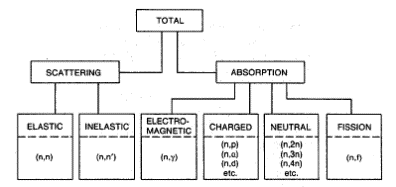
\includegraphics[scale=0.55]{image1.png}
\end{center}
\subsection{Subdivision en escalier}
Une \textbf{subdivision} $P$ d'un intervalle $[a, b]$ est un ensemble \textbf{fini} de points appartenant à cet intervalle. Si $P'$ est une subdivision de $P$ on dira que \textbf{$P'$ est un raffinement de $P$}.\\

Une \textbf{fonction en escalier} est une fonction $\phi$ tel qu'il existe une subdisiviant de $P$ ou $\phi$ est constante sur tout sous-intervalle ouvert.

\subsection{Intégrale d'une fonction bornée}
On peut définir, comme pour les limites, des intégrales supérieures et inférieure. Si $\psi$ majore $f$ et $\phi$ minore $f$, on peut écrire :
$$\int_{[a,b]} \phi \leq \int_{[a,b]} \psi$$

\subsection*{Définition}
$f$ est \textbf{intégrable} (au sens de Riemann) sur $[a, b]$ ssi  (les notations définissent l'intégrale inférieure et supérieure)
$$\underline{\int_{[a,b]}} f = \overline{\int_{[a,b]}} f$$
\textit{Wikipédia : On dit que f est intégrable (au sens de Riemann) ou Riemann-intégrable, lorsque son intégrale inférieure et son intégrale supérieure sont égales, et cette valeur commune est alors appelée l'intégrale de Riemann de f.}\\

\textbf{CNS d'intégrabilité} : f est intégrable sur [a,b] ssi il existe une suite ($\phi_n$) de fonction en escalier minorant f est une suite ($\psi_n$) de fonction en escalier majorant $f$ telle que : 
$$\lim\limits_{\substack{n \to \infty}} \left(\int_{[a,b]} \phi_n - \int_{[a,b]} \psi_n \right) = 0$$

\subsection{Sommes de Darboux}
Pour $f$, on associe à toute subdivision $P$ deux fonction en escalier : $\psi_P$ (:= sup f(x)) et $\phi_P$ (:= inf f(x)).\\
On définit de cette manière la petite somme de Darboux $s(P)$
$$s(P) := \int_{[a,b]} \phi_P(x) dx$$
et la grande somme de Darboux
$$s(P) := \int_{[a,b]} \psi_P(x) dx$$
\begin{wrapfigure}[6]{l}{3cm}
	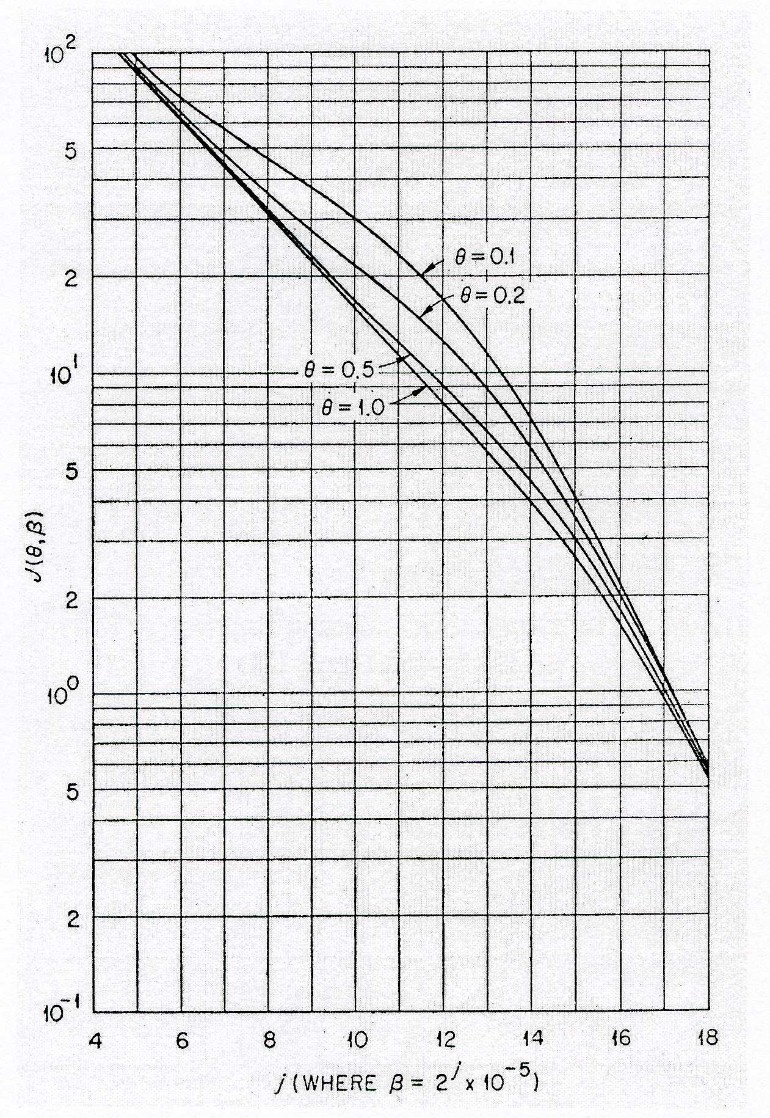
\includegraphics[width=3cm]{image2.jpg}
\end{wrapfigure}
L'idée est d'approcher l'aire de la courbe (voir ci-contre) en prenant des $s(P)$ et $S(P)$ de plus en plus proche.\\

\textbf{CNS d'intégrabilité via les sommes de Darboux :} Une fonction $f$ bornée sur $[a,b]$ est intégrable sur $[a,b]$ ssi $\forall \epsilon > 0$ il existe une subdivision $P$ telle que : $S(p) - s(P) < \epsilon$.

\subsection{Convergence des sommes de Riemann}
Sous quelle condition une suite de sommes de Riemann tend-elle vers l'intégrale et quelle est l'erreur commise par cette approche?\\

\textbf{Proposition "convergence des sommes de Riemann"} : $f$ est intégrable sur $[a,b] \Leftrightarrow$ pour toute suite de subdivision pointée de $[a,b]$ de norme $\rightarrow 0$, la suite des sommes de Riemann converge.\\

\textbf{Proposition "majoration de l'erreur"} : voir \textit{page 12}.

\section{Propriétés de l'intégrale simple}
\subsection{Additivité relativement au domaine d'intégration}
Soit $f = [a,b] \rightarrow \mathbb{R}$ et $a < c < b$ ;
$$\int_{[a,b]} f = \int_{[a,c]} + \int_{[c,b]} f$$

\subsection{Fonctions monotones}
Si $f : [a,b] \rightarrow \mathbb{R}$ est monotone, alors $f$ est intégrable sur $[a,b]$.

\subsection{Fonctions continues}
Si $f : [a,b] \rightarrow \mathbb{R}$ est continue, alors $f$ est intégrable sur $[a,b]$.

\subsection{Fonctions continues par morceaux}
Si $f$ n'est définie que sur \underline{l'intervalle ouvert} $]a,b[$, on peut définir $\int_a^b$ de la manière suivante : On prolonge $f$ en $\tilde{f}$ := $f(x)\ si\ x \in ]a,b[$ et $0\ si\ x = a\ ou\ b$.\\

Ainsi, $f$ \textbf{est intégrable sur} $]a,b[$ ssi $\tilde{f}$ l'est sur $[a,b]$, et dans ce cas
$$\int_{]a,b[} = \int_a^b f = \int_{[a,b]} \tilde{f}$$
\textbf{Attention :} $f$ doit impérativement être \textbf{bornée} sur $]a,b[$ sinon $\tilde{f}$ ne l'est pas.\\

\textit{Toute fonction continue par morceaux sur $[a,b]$ est bornée est intégrable.}

\subsection{Intégrabilité versus domaine de discontinuité}
Peut-on intégrer des fonctions contenant des points de discontinuité ? \\

\textbf{Théorème :} Une fonction $f$, \underline{bornée} sur $[a,b]$ est Riemann-intégrable sur $[a,b]$ \textbf{ssi} l'ensemble des points de discontinuité de $f$ est de \textit{"longueur nulle"}.

\subsection{Linéarité de l'intégration sur $[a,b]$} 
Je pense qu'avec Algèbre, c'est assez clair.

\subsection{Intégrabilité de composées, produits, valeur absolue}
Si $f([a,b] \subseteq [c,d]$, $f$ est intégrable sur $[a,b]$ et $g \in C^0([c,d])$ alors $g \circ f$ est intégrable sur $[a,b]$.\\

\textbf{Propriétés :}
\begin{enumerate}
	\item Si $f$ est intégrable sur [a,b], alors $f^2$ est intégrable sur [a,b] (Dem. )
	\item Si $f$ et $\tilde{f}$ sont intégrables sur [a,b], alors $f . \tilde{f}$ est intégrable sur [a,b].
	\item Si $f$ est intégrable sur [a, b], alors $|f|$ l'est aussi.
\end{enumerate}
\textbf{Démonstrations associées}
\begin{enumerate}
	\item Il suffit de remarquer que $f^2 = g \circ f$ où $g : y \rightarrow y^2$ et appliquer la proposition.$\square$
	\item Il suffit de remarquer que $f . \tilde{f} = \frac{1}{4}(f + \tilde{f}) - \frac{1}{4}(f - \tilde{f})^2$ et d'appliquer la proposition .$\square$
	\item SIl suffit d'appliquer la proposition précédente à $g \circ f$ où $g : y \rightarrow |y|$.$\square$
\end{enumerate}

\subsection{Croissance de l'intégration sur $[a,b]$}
\textbf{Théorème de comparaison :} Soient $f, \tilde{f}$, intégrables sur $[a,b]$ : $f \leq \tilde{f}$ sur $[a, b] \Rightarrow \int_a^b f \leq \int_a^b \tilde{f}$.\\

\textbf{Corolaire 1 :} Si $f \geq 0$ sur [a,b] alors $\int_a^b f \geq 0$.\\

\textbf{Corolaire 2 :} Soit $f$ intégrable sur [a,b] et $m, M \in \mathbb{R}$ tels que $\forall x \in [a, b] : m \leq f(x) \leq M$. Alors : $m(b-a) \leq \int_a^b f \leq M(b-a)$.\\

\textbf{Corolaire 3 :} $|\int_a^b f| \leq \int_a^b |f|$.

\begin{proof}\ \\
	Appliquons la croissance de l'opérateur $\int_a^b$ à :
	$$-|f| \leq f \leq |f|$$
	Ce qui donne, grâce à la linéarité de l'opérateur $\int_a^b$ :
	$$- \int_{[a,b]} |f| = \int_{[a,b]} -|f| \leq \int_{[a,b]} f \leq \int_{[a,b]} |f|$$
\end{proof}

\textbf{Corolaire 4 :} $|\int_{[a,b]} f| \leq sup\ |f|.(b-a)$. \\
\textit{La valeur absolue de l'intégrale de $f$ sur un intervalle $I$ est majorée par le produit de la longueur de I et du suprémum de la valeur absolue de $f$ sur $I$.}

\subsection{Théorème de la moyenne (du calcul intégral)}
La \textbf{valeur moyenne} de $f$ sur $[a,b]$ est  :
$$\frac{\int_a^b f}{b-a} = \frac{\int_a^b f}{\int_a^b 1} = \frac{Intégrale}{Longueur([a,b])}$$
\textbf{Théorème :} Si $f$ est continue sur $[a,b]$, alors il existe $\xi \in ]a,b[$ tel que :
$$\int_a^b f = \underbrace{f(\xi)(b-a)}_{*}$$
$* = valeur\ moyenne\ de\ f\ sur\ [a,b]$.\\
Autrement dit : 
$$\exists c : f(c) = f_{moy} := \frac{\int_{[a,b]} f}{b-a}$$

\subsection{Intégrale nulle - Intégrande nulle ?}
Toute fonction continue et positive de moyenne nulle sur $[a,b]$ est nulle sur [a,b].
\begin{center}
	$\int_a^b f = 0$, $f \geq 0$ sur $[a,b]$ et $f$ continue sur $[a,b]$\\
	$\Rightarrow f = 0\ sur\ [a,b]$
	
\end{center}

\section{Théorème fondamental du CDI}
\subsection{Continuité et dérivation d'intégrales définies}
Soit $f$ intégrable sur $[a,b]$, et soit $c \in [a,b]$.\\
Si $F(x) := \int_c^x f$ pour tout $x \in [a,b]$, alors :
\begin{enumerate}
	\item $F(x)$ est continue
	\item Si $f$ est continue sur $[a,b]$, alors $F$ est dérivable et $F' = f$.
\end{enumerate}
\textbf{Corolaire}
\begin{enumerate}
	\item Si $f$ est continue sur $[a,b]$, alors $\int_a^x f$ est une primitive de $f$ sur $[a,b]$.
	\item Toute fonction continue admet une primitive.
\end{enumerate}
Notons que la fonction après intégration n'est pas forcément continue.\\

Si $f$ \textbf{est continue}, on peut en déduire de ce corolaire : 
$$\frac{d}{dx}\int_c^x f = f(x)$$

\subsection{Règles de Leibniz}
Partant de la déduction du corolaire précédent, on peut écrire : 
$$\frac{d}{dx}\int_c^{g(x)} f = f|_{g(x)}.g'(x)$$

\begin{proof}
	\ \\ Posons $\mathbb{F} = \int_c^x f$\\
	On a donc : 
	$$\frac{d}{dx}\mathbb{F} = f(x)$$
	$$\Rightarrow \frac{d}{dx}\mathbb{F}(g(x)) = f|_{g(x)}.g'(x)$$
\end{proof}
La bonne nouvelle, c'est que ça fonctionne aussi avec des fonctions : 
$$\frac{d}{dx}\int_{h(x)}^{g(x)} f = f|_{g(x)}.g'(x) - f|_{h(x)}.h'(x)$$

\subsection{Théorème fondamental du CDI}
Si : 
\begin{enumerate}
	\item $f$ est intégrable sur $I \subseteq \mathbb{R}$
	\item $F' = f$ sur $I$
\end{enumerate}
Alors 
$$\int^x_c f = F(x) - F(c)$$

\textbf{Corolaire} (mêmes hypothèses)
$$\forall x_0 \in [a,b]\ \ x \mapsto \int^x_{x_0} f\ \ \ est\ une\ primitive\ de\ f\ sur\ [a,b]$$

\section{Formules de substitution et d'intégration par partie}
Seulement des applications en TP.

\section{Longueurs, aires, volumes par intégrales simples}
Juste vu le point \textit{9.4.4 La trompette de Torricelli} qui est à titre "informatif".

\section{Intégrales sur un pavé}
\subsection{Intuitions géométriques et pondérée}
En toute rigueur, on ne peut pas a priori savoir ce qu'est le volume, la "masse totale".

\subsection{Subdivision du domaine}
On va découper le domaine en pleins de petits carrés élémentaires pour formé une \textit{subdivision cartésienne} du domaine.

\subsection{Petites et grandes sommes de Darboux}
Comme précédemment, on défini la \textbf{petite somme de Darboux} :
$$s_p := \sum_k m_k\mu_2(P_k)$$
Rappelons que pour une même subdivision $P$, la petite somme de Darboux est toujours inférieure ou égale à la grande somme de Darboux ($\mu_2$ correspond à l'aire). \\

En procédant par raffinement, les petites sommes vont augmenter et les grandes diminuer jusqu'à obtenir les intégrales supérieures et inférieures de notre fonction.

\subsection{Définition de l'intégrale de $f$ sur $P$}
\textsc{Définition :} $f$ est \textbf{intégrable} \textbf{sur $P$} 
$$\Leftrightarrow \forall \epsilon > 0: \exists P\ subdivision\ de\ P\ telle\ que\ S_P - s_p < \epsilon$$
Il s'agit la d'une condition nécessaire et suffisante d'intégrabilité. On peut la reformuler comme suit : 
$$\sum_k(M_k - m_k)\mu_2(P_k) < \epsilon$$

\subsection{Sommes de Riemann et norme d'une subdivision}
Dans chaque rectangle $P_k$, on va choisir un point $(\xi_k, \eta_k)$ telle que la somme
$$\sum_k f(\xi_k, \eta_k)\mu_2(P_k)$$
est trivialement une somme de Riemann associée à P ; On peut la faire tendre vers l'intégrale (subdivision de normes tendant vers zéro)

\subsection{Intégrales triples, intégrales multiples}
$$\iiint_P f(\vec{x})d\vec{x}$$

\subsection{Intégrales multiples dans un domaine $nD$}
C'est pareil !
$$\iiint...\iiint$$ 

\section{Intégrales emboîtées}
\subsection{Deux intégrales emboitée}
La notation est la suivante : 
$$\int_c^d \int_a^b f(x, y) dx dx := \int_c^d A(y) dy$$

\subsection{Théorème de Fubini sur un rectangle}
Soit $f : [a,b] \times [c,d] \rightarrow \mathbb{R}$ une fonction bornée et intégrales. Alors :
$$\iint_P f = \int_a^b\underbrace{\left(\int_c^d f(x_{fixé}, y) dy\right)}_{indép\ de\ y}dx$$
et
$$\iint_P f(x,y) dxdy = \int_c^d\underbrace{\int_a^b f(x, y_{fixé}) dx}_{indép\ de\ y}dy$$

Plus formellement : 
$$\iint_{[a,b] \times [c,d]} f = \int_{[a,b]} dx \int_{[c,d]} f(x,y) dy$$
$$= \int_{[c,d]} dy \int_{[a,b]} f(x,y) dx.$$

Ce théorème ramène une intégrale sur un pave $\mathbb{R}^2$, c'est à dire sur une intégrale double.

\subsection{Cas ou Fubini ne s'applique pas}
Le théorème ne s'applique pas lorsque les deux intégrales simples existent, mais pas l'intégrale double.\\

\textbf{Corolaire}\\
Si $f$ est \textbf{intégrable sur le pavé, alors} les intégrales commutent.

\subsection{Théorème de Fubini sur un pavé $nD$}
Il y à dès lors $!n$ ordres d'intégration possibles.

\section{Intégrales sur une région mesurable}
\subsection{Mesure nulle selon Riemann}
$A$ est de \textbf{$n-$mesure nulle au sens de Riemann} ssi $inf_P S_P(A) = 0$.\\

Dans $\mathbb{R}^n (n \geq 2)$, tout chemin rectifiable est d'aire nulle (selon Riemann). Une courbe est donc de longueur finie mais d'aire nulle.

\subsection{Mesure selon Riemann}
La \textbf{$n-$mesure} selon Riemann de $G$ existe et est notée $\mu_n(G) \Leftrightarrow$
$$inf\ S_P(G) = sup\ s_P(G) =: \mu_n(G)$$

\subsection{Intégrabilité des fonctions continues}
\textbf{Proposition}
\begin{center}
	Soit $G \subseteq \mathbb{R}^2$ un compact dont la frontière $fr\ G$ est d'aire nulle (selon Riemann). Si $f$ est continue sur $G$, alors $f$ est intégrable sur $G$.
\end{center}

\subsection{Intégrales sur des domaines inclus dans $\mathbb{R}^n$}
Les deux sections précédentes s'étendent de manière évidente à la dimension $n$.

\subsection{Contribution d'un ensemble de mesures nulles}
Si $g = f$ sur $G$ sauf une partie de $n-$mesure = 0, alors $g$ est intégrables et 
$$\int_G g = \int_G f$$

\section{Théorème de Fubini sur une région de $\mathbb{R}^n$}
\subsection{Région normales dans $\mathbb{R}^2$}
Une région est dite normale par rapport à $y$ ssi : $a \leq x \leq b$ et $h_1(x) \leq y \leq h_2(x)$ où $h_i \in C^0$. (Une région normale doit être connexe).

\subsection{Théorème de Fubini sur domaine normal 2D}
Si $f$ est bornée et intégrable sur une région normale $G$ telle que $\forall x \in [a,b] : y \rightarrow f(x,y)$ est intégrable, alors :
$$\iint_G f(x,y) dx dy = \int_a^b\int_{h_1(x)}^{h_2(x)} f(x,y) dy dx$$

\begin{proof}\ \\
	Soit $G$ compris dans un pavé cartésien $P = [a,b] \times [c,d]$. Par Fubini sur pavé : 
	$$\iint_{[a,b]\times [c,d]} f_p = \int_a^b \left( f_p(x,y) dy\right) dx$$
	$$= \int_a^b \left( \int_{h_1(x)}^{h_2(x)} f(x,y) dy \right)dx$$
\end{proof}

\subsection{Calcul d'aires planes : Fubini confirme}
L'aire sous la courbe est toujours vérifiée avec Fubini :
$$aire(G) := \iint_G 1 = \int_a^b \left( \int_{h_1(x)}^{h_2(x)} 1\ dy \right)dx = \int_a^b \left( h_1(x) - h_2(x)\right) dx$$

\subsection{Applications de Fubini dans $\mathbb{R}^2$}
Méthode à suivre en TP, \textit{cf. page 71}.

\subsection{Théorème de Fubini par sections planes dans $\mathbb{R}^3$}
Le principe est toujours le même : on découpe le domaine en différente tranche pour passer de $\iiint$ à $\iint$.

$$\iiint_G f(x,y,z)dx dy dz = \int_{z_1}^{z_2} \left( \iint_{G_z} f(x, y, z) dx dy \right) dz$$


\subsection{Théorème de Fubini par sections rectilignes dans $\mathbb{R}^3$}
C'est d'ici que vient le nom \textit{spaghettis de Fubini}. On découpe une aire par des sectins de droites parallèle à l'axe $oz$.\\
Pour rappel, une région $G$ de $\mathbb{R}^3$ est normale par rapport à $z$ si elle peut être décrite par les inégalités : $(x,y) \in D)$, $z_1(x,y) \leq z \leq z_2(x,y)$\\

Le théorème pour les régions normales :
$$\iiint_G f(x,y,z) dx dy dz = \iint_D \underbrace{\left(\int_{z_1(x,y)}^{z_2(x,y)}f(x,y, z) dz\right)}_{indep.\ de\ z} dxdy$$

Le domaine $D$ est la projection de $G$ sur $Oxy$.


\section{Propriétés des intégrales multiples}
\subsection{Additivité de l'intégration d'une même fonction}
Si $G_1$ et $G_2$ sont deux compacts à frontières $n-$négligeable dans $\mathbb{r}^n$, dont les intérieurs sont disjoints, alors : 
$$\int_{G_1} f + \int_{G_2} f = \int_{G_1 \cup G_2} f$$

\subsection{Linéarité de l'intégration sur un même domaine}
L'ensemble des fonctions bornées $f : G \subseteq \mathbb{R}^n \rightarrow \mathbb{R}$ et intégrable sur $G$ forme un espace vectoriel réel $V$. Ainsi, l'opérateur d'intégration est linéaire de $V$ dans $\mathbb{R}$.

\subsection{Croissance de l'opérateur $\int_G$}
Si $\forall \vec{x} \in G : f(\vec{x}) \leq \tilde{f}(\vec{x})$ alors
$$\int_G f \leq \int_G \tilde{f}$$

\subsection{Une norme sur $C^0$}
Pas vu en cours ! :)

\subsection{Théorème de la majoration d'intégrales}
Si $f$ et $g$ sont intégrables sur $G$ et si $g \geq 0$ sur $G$ alors : 
$$(inf\ f)_G \int_G g \leq \int_G (fg) \leq (sup\ f)_G \int_G g$$
La démonstration se fait par pincement en partant de $inf_G\ f \leq f \leq sup_G\ f$ ($\forall \vec{x} \in G$).

\subsection{Valeur moyenne, théorème de la valeur moyenne}
Si $G$ est un compact connexe par arcs à frontière $n-$négligeable dans $\mathbb{R}^n$ et si $f$ est continue sur $G$ alors 
$$\exists x \in int\ G : f(x) = \frac{\int_G f}{\mu_n(G)}$$
(Démonstration page \textit{87} du syllabus).


\section{Changement de variables dans les intégrales multiples}
Cette partie est essentiellement pratique, elle sera vue en long et en large aux TP's! 



%%%%%%%%%%%%%%%%%
% Bibliographie %
%%%%%%%%%%%%%%%%%
%\newpage
%\chapter{Bibliographie}
%\nocite{*}
%\printbibliography[heading=none]

%%%%%%%%%%%
% Annexes %
%%%%%%%%%%%
\appendix
%\input{annexes/annexe1.tex}


\end{document}


